\section*{New Clock Stability Application}

\gpstkapp{Clock Tools}, a recent addition to the GPSTk, allows for
basic clock stability analyses.  \gpstkapp{Clock Tools} implement
clock time-domain frequency stability metrics as well as data editing,
noise identification, and plotting routines.  The \gpstkapp{Clock
  Tools} are interoperable with other GPSTk programs, allowing clock
analyses to be easily run alongside other GPS analyses.

Given RINEX GPS observation and navigation files, clock estimates may
be generated using the GPSTk \gpstkapp{Observed Range Deviation (ORD) Tools}.
Kalman filter and time interval analyzer data-sets provide another
source of clock data.  For instance, the TSC 5110A Time Interval
Analyzer (TIA) compares two input clocks and outputs the phase
difference between them at a 10- to 100-Hz sampling rate.  These clock
estimates are used for time-domain frequency stability analysis.

Frequency stability measures the ability of a clock to maintain its nominal frequency over a given period of time.  From input clock data, both short-term and long-term stability can be assessed.  The Allan variance represents the variance of a clock from its nominal value over a range of averaging times.  The Allan variance is an IEEE standard for stability analysis~\cite{ieee1139}.  An Allan variance plot is often helpful in stability analysis.

The \gpstkapp{Clock Tools} suite currently computes the Allan, overlapping Allan, modified Allan, total Allan, overlapping Hadamard, and dynamic Allan deviation stability metrics.  These \gpstkapp{Clock Tools} may be run from the command line with their output piped to other GPSTk programs.  Data formatting and outlier removal routines for GPS and time interval analyzer data-sets facilitate compatibility with the \gpstkapp{Clock Tools} stability programs.

\subsection*{Design}

The \gpstkapp{Clock Tools} applications are encapsulated, so that the output of
one tool acts as the input to the next.  By using redirection and
piping the user is able to connect the \gpstkapp{Clock Tools} together in a way
that allows for flexibility in analysis and ease of use.

Routines within the \gpstkapp{Clock Tools} suite fall into four functional categories: input parsing, data grooming, data analysis, and plotting.  Input parsing takes data generated outside of \gpstkapp{Clock Tools} and puts it in a format understood within the suite.  Data grooming cleans the data of outliers before analysis.  Data analysis performs the frequency stability calculations.  Plotting creates a graphical representation of the frequency stability.

\subsection*{Implementation}

As mentioned, \gpstkapp{Clock Tools} has four functional categories: input
parsing, data grooming, data analysis, and plotting.
Table~\ref{table:clockapps} presents a description and example use of
each tool.  Note that \gpstkapp{ordClock} makes an estimate of the receiver’s
clock offset by averaging the ORDs of all the GPS satellites at each
epoch.  An epoch is an instant in time in which GPS data is recorded.
%
\begin{table*}
\centering
\caption{Description and example invocations of \gpstkapp{Clock Tools}.}
\label{table:clockapps}
\begin{tabular}{lll} \hline \hline
\emph{Tool} & \emph{Description} & \emph{Example} \\ \hline
\gpstkapp{ORDPhaseParser} & Parses data generated by the \gpstkapp{ORD Tools} & \gpstkcommand{ordGen –o input.o –e input.n | } \\ 
 & &\gpstkcommand{ordClock|ORDPhaseParser>parsed.dat} \\ \hline
\gpstkapp{TIAPhaseParser} & Parses data generated by the & \gpstkcommand{TIAPhaseParser < raw.dat > parsed.dat} \\ 
   &  TSC 5110A Timing Interval Analyzer. & \\ \hline 
\gpstkapp{rmoutlier} & Removes outlier data within a set of  data. & \gpstkcommand{rmoutlier < parsed.dat} \\ \hline 
\gpstkapp{nallandev} & Computes the Allan deviation. & \gpstkcommand{nallandev < parsed.dat} \\ \hline 
\gpstkapp{oallandev} & Computes the overlapping Allan deviation. & \gpstkcommand{oallandev < parsed.dat} \\ \hline 
\gpstkapp{mallandev} & Computes the modified Allan deviation. & \gpstkcommand{mallandev < parsed.dat} \\ \hline 
\gpstkapp{totvar} & Computes the total Allan deviation. & \gpstkcommand{totvar < parsed.dat} \\ \hline 
\gpstkapp{ohadamarddev} & Computes the overlapping Hadamard & \gpstkcommand{ohadamarddev < parsed.dat} \\
& deviation. & \\ \hline
\gpstkapp{dallandev} & Computes the dynamic Allan deviation. & \gpstkcommand{dallandev < parsed.dat} \\ \hline 
\gpstkapp{allanplot} & Plots the output of \gpstkapp{nallandev}, \gpstkapp{oallandev}, & \gpstkcommand{nallandev < parsed.dat | allanplot} \\ 
& \gpstkapp{ohadamarddev}, \gpstkapp{totvar}, and \gpstkapp{mallandev}. & \\ \hline 
\gpstkapp{ddevplot.m} & Plots the output of dallandev. & \gpstkcommand{octave ddevplot.m} \\ \hline \hline
\end{tabular}
\end{table*}
%
The input parsers are the classes \gpstkapp{ORDPhaseParser} and
\gpstkapp{TIAPhaseParser}.  The data grooming tool is
\gpstkapp{rmoutlier}.  The data analysis tools are
\gpstkapp{nallandev}, \gpstkapp{oallandev}, \gpstkapp{mallandev},
\gpstkapp{totvar}, \gpstkapp{ohadamarddev}, and \gpstkapp{dallandev}.
The plotting scripts are \gpstkapp{allanplot} and
\gpstkapp{ddevplot.m}.  Data flows from the parsers to data grooming
to data analysis and finally to plotting.

\subsection*{Example Usage and Plots}

Two example command lines are given below.  The first command
generates clock estimates using the GPSTk ORD tools (\gpstkapp{ordGen} and
\gpstkapp{ordClock}), parses the data (\gpstkapp{ORDPhaseParser}), then removes outliers
(\gpstkapp{rmoutlier}), computes the overlapping Allan deviation (\gpstkapp{oallandev}), and
finally writes the data to a file (\gpstkcommand{output.oadev}).  The second example
takes data in from a file produced by the Timing Interval Analyzer
(\gpstkcommand{raw.dat}), parses the data (\gpstkapp{TIAPhaseParser)}, computes the overlapping
Hadamard variance (\gpstkcommand{ohadamard}), and plots the output (\gpstkcommand{allanplot}).
%
\begin{scriptsize}
\begin{lstlisting}
ordGen –o input.o –e input.n | ordClock 
| ORDPhaseParser | rmoutlier | 
oallandev > output.oadev

raw.dat | TIAPhaseParser | 
ohadamard | allanplot
\end{lstlisting}
\end{scriptsize}
%
Another example is shown below.  This example is an analysis performed on a reference station that is part of the NGA GPS Monitor Station Network (MSN).

This analysis compares the results of running an overlapping Allan
deviation calculation on data generated by \gpstkapp{ordClock} from
unsmoothed raw RINEX files versus data output by the NGA Kalman
filter. The \gpstkapp{ordClock} and Kalman filter data sets cover
different time periods, but both data sets are good representatives of
nominal MSN data. The overlapping Allan deviation of the \gpstkapp{ordClock}
generated data is represented by the blue line.  The overlapping Allan
deviation of the Kalman filter generated data is represented by the
green line.  The lighter slanted red line shows the 5071A CFS
time-domain stability specification.  The darker red line along the
bottom represents the cesium’s flicker floor.  Note that drift removal
may be necessary depending on the input dataset and the deviation
computation performed.
%
\begin{figure*}
  \centering
  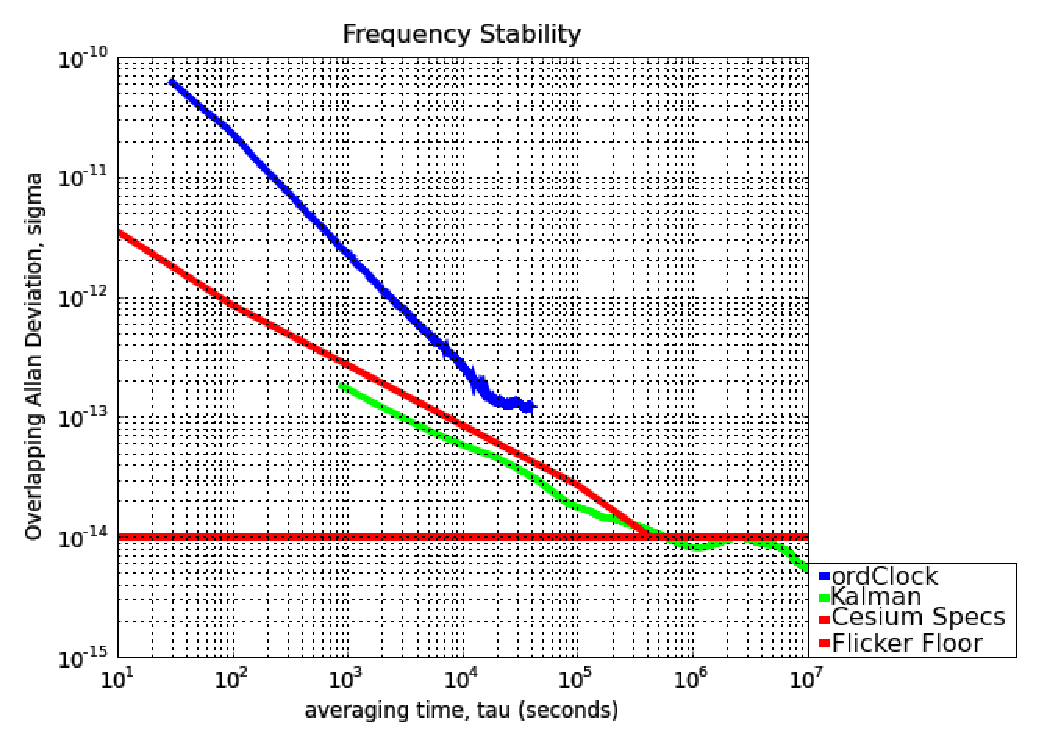
\includegraphics[width=5in,bb=65 387 547 727]{clockapps.eps}
  \caption{Frequency Stability of \gpstkapp{ordClock} and Kalman Filter Data}
  \label{fig:clockapps}
\end{figure*}
%
Figure~\ref{fig:clockapps} shows that the frequency stability of the
clock estimates generated by the Kalman filter lies within the CFS
specifications, but that the frequency stability of the output
generated by \gpstkapp{ordClock} from the raw data does not.  Using
raw GPS data and \gpstkapp{ordClock} a stability trend is apparent,
but further filtering and smoothing of the data is necessary to get
more accurate clock stability estimates.
